

%%%%%%%%%%%%%%%%%%%%%%%%%%%%%%%%%%%

\begin{frame}
\frametitle{Filtros Paso Todas}

\vspace{-0.2cm}



\begin{itemize}
\footnotesize
\item Un filtro paso todas cumple que : $|H(e^{jw})|=1 \:\: \forall w$

\visible<2->{

\item Un filtro IIR con coeficientes reales y causal de la forma

$H(z)=\pm \frac{d_M + d_{M-1}z^{-1}+\dots+ z^{-M}}{1+d_1z^{-1}+\dots+ d_M z^{-M}}=\pm \frac{z^{-M}D_M(z^{-1})}{D_M(z)}$

\hspace{4cm}$D_M(z)=1+d_1 z^{-1}+\dots + d_M z^{-M}$


}

\visible<3->{

\item Es por construcción un filtro paso todas:

$|H(e^{jw})|^2\!=\!H(e^{jw})H(e^{-jw})\!=\!H(z)H(z^{-1})|_{z=e^{jw}}\!=\!(\pm)^2 \frac{z^{-M}D_M(z^{-1})}{D_M(z)} \frac{z^{M}D_M(z)}{D_M(z^{-1})}=1$

}

\visible<4->{

\item $z_{POLO}=re^{j\theta}  \leftrightarrow z_{CERO}=\frac{1}{r}e^{j\theta}$

\item Si el filtro es estable $\rightarrow$ tiene sus polos (raíces de $D_M(z)$) dentro del círculo unidad y sus ceros (raíces de $D_M(z^{-1})$) fuera del círculo unidad. Los polos y los ceros se encuentran enfrentados con una simetría especular respecto al círculo.

}

\visible<5->{

\item Como no atenúan ninguna frecuencia, son útiles para modificar el desfase introducido por otros filtros. 

}

\visible<6->{

\item El desfase total introducido por el filtro paso todas H(z) entre las frecuencias $w\in[0 ,\pi]$ es de $M\pi$. 

}
\end{itemize}
\end{frame}

\begin{frame}
\frametitle{Ejemplo Filtros Paso Todas}
\footnotesize

\color{olivegreen} Comprobar el comportamiento del filtro $H(z)= \frac{z^{-M}D_M(z^{-1})}{D_M(z)}$, con 
$D_M(z)=1+0.4 z^{-1}+0.18z^{-2}-0.2z^{-3}$

\color{gray}

\begin{columns}[c]
\begin{column}{4cm}
\lstinputlisting{./Matlab/EjPasoTodos.m}
\end{column}
\begin{column}{5cm}
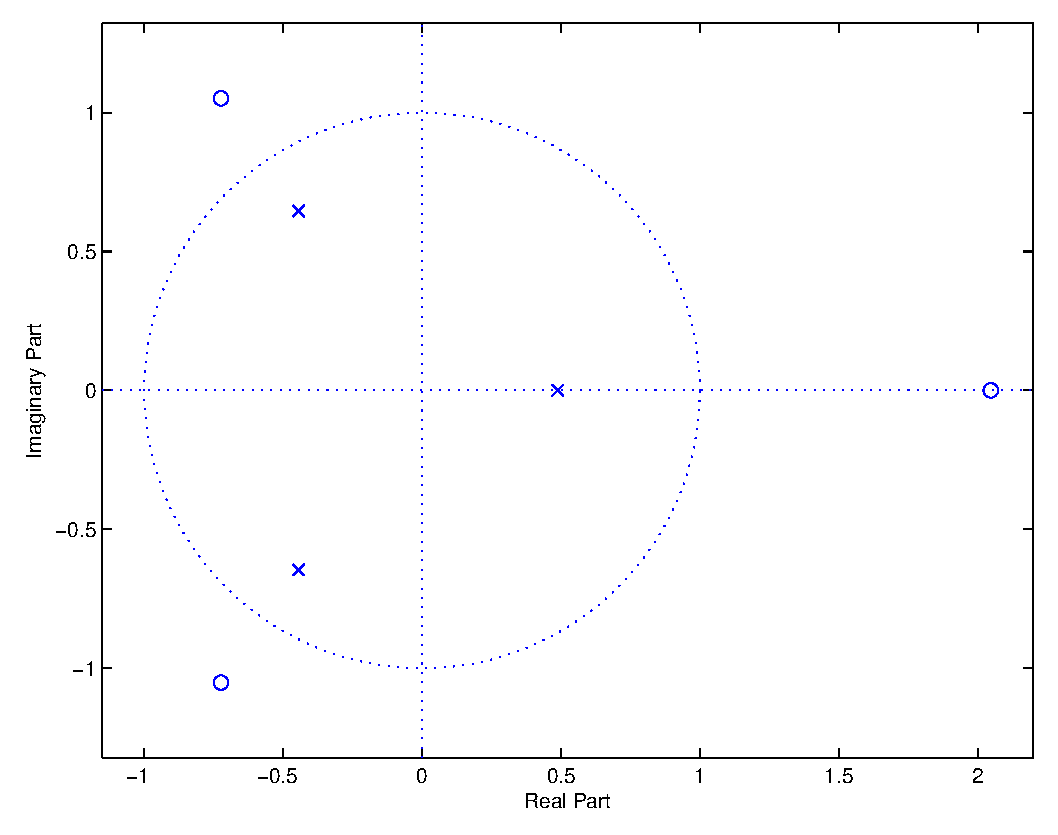
\includegraphics[width=4cm]{./Figures/EjPasoTodo1.eps}

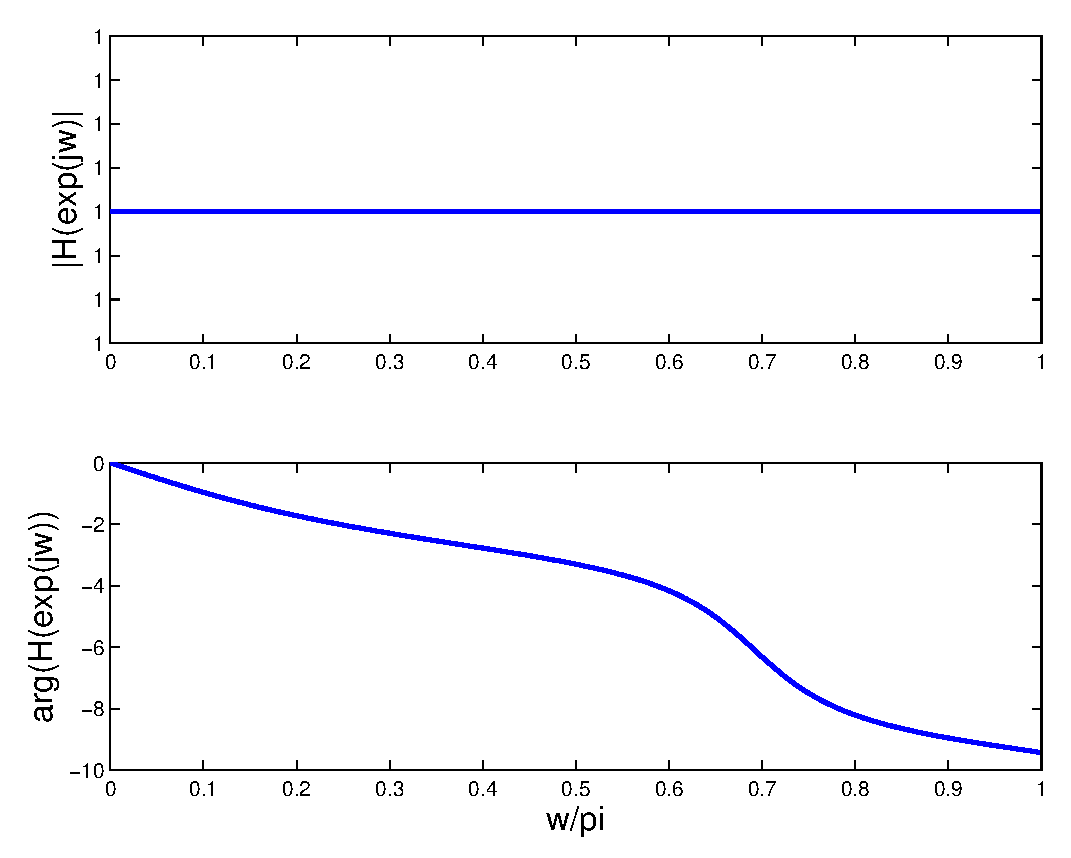
\includegraphics[width=4cm]{./Figures/EjPasoTodo2.eps}
\end{column}
\end{columns}


\end{frame}
